\documentclass{sintefbeamer}

% packages, font, color, and newcommands
\usepackage{amsfonts, amsmath, oldgerm, lmodern, bm}
% \usepackage[font={footnotesize}]{caption}
\usepackage{natbib}
\usepackage{url}
\usepackage{tikz}
\usepackage{amssymb}
\usepackage{amsmath}
\usepackage{amsthm}
\usepackage{mathrsfs}
\usepackage{empheq}
\usepackage{mdframed}
\usepackage{bm}
\usepackage{animate}
\usepackage{xcolor,colortbl}
\usepackage{graphicx}
\bibliographystyle{apalike}
\usefonttheme{serif}
\usetikzlibrary{arrows.meta,
                chains,
                calc,
                positioning,
                shapes.geometric,
                backgrounds}

\title{Mathematical modeling of emulsions}
\subtitle{}
\author{\href{http://basilisk.fr/sandbox/fintzin/Rising-Suspenion/RS.c}{\underline{N. Fintzi}\footnote{IFP \'Energies Nouvelles, France}$^{,2}$}, JL. Pierson$^1$ and S. Popinet\footnote{Sorbonne Universit\'e, France}}
% \date{Created on May 22, 2022}

\titlebackground{image/800good.png}

% document body
\addtobeamertemplate{navigation symbols}{}{%
    \usebeamerfont{footline}%
    \usebeamercolor[fg]{footline}%
    % \hspace{1em}%
    % \vspace{1em}%
    \insertframenumber/\inserttotalframenumber
}
\usepackage{stmaryrd}

\usepackage{amsmath}


\begin{document}
\maketitle

\begin{frame}
  \frametitle{Industrial context and motivation: Liquid-Liquid separation process}
  % \begin{figure}[h!]
liquid-liquid extraction is an economical alternative for separating compounds that are difficult to separate by distillation

\centering
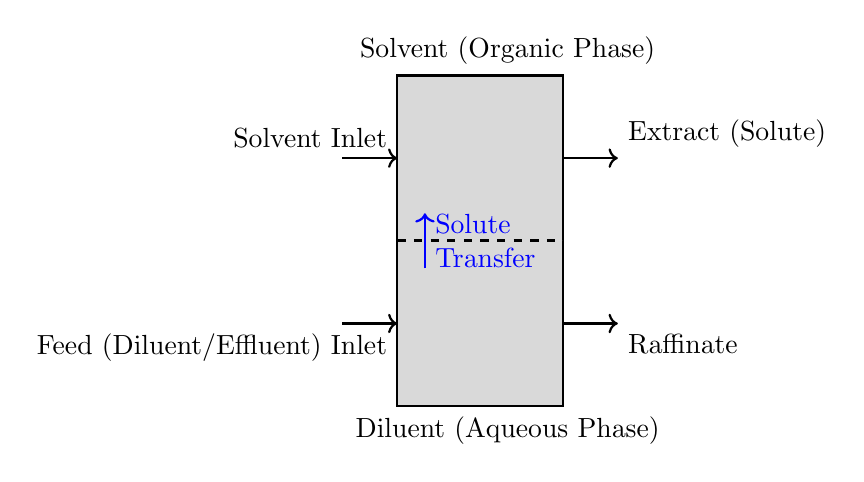
\begin{tikzpicture}[scale=0.7,very thick]

  % Draw the container
  \draw[fill=gray!30,thick] (0,0) rectangle (3,6);
  \draw[fill=gray!30,dashed] (0,3) -- (3,3); % Separation line
  
  % Labels for phases
  \node[anchor=south] at (2,6) {Solvent (Organic Phase)};
  \node[anchor=north] at (2,0) {Diluent (Aqueous Phase)};
  
  % Draw solute transfer
  \draw[->,thick,blue,text width=1.5cm] (0.5,2.5) --++ (0,1) node[midway,right] {Solute Transfer};
  
  % Inlet arrows
  \draw[->,thick] (-1,4.5) -- (0,4.5) node[anchor=south east] {Solvent Inlet};
  \draw[->,thick] (-1,1.5) -- (0,1.5) node[anchor=north east] {Feed (Diluent/Effluent) Inlet};
  
  % Outlet arrows
  \draw[->,thick] (3,4.5) --++ (1,0) node[anchor=south west] {Extract (Solute)};
  \draw[->,thick] (3,1.5) --++ (1,0) node[anchor=north west] {Raffinate};
  
  \end{tikzpicture}

\end{frame}
\begin{frame}
  \frametitle{Industrial context and motivation: Liquid-Liquid separation process}
  % \begin{figure}[h!]
% liquid-liquid extraction is an eco  nomical alternative for separating compounds that are difficult to separate by distillation

    \centering
    % \pause 
    \includegraphics[height=0.4\textwidth]{image/liq-liq_LE_auto_x5.jpg}
    \includegraphics[height=0.4\textwidth]{image/scheme_liq-liq_mieux.png}
    % \pause 
    \includegraphics[height=0.4\textwidth]{image/process_LE_auto_x4.jpg}
    % \includegraphics[height=0.15\textheight]{image/bubbles.png}
  %   \caption{
  %     (Left)   Pilot-scale illustration of the agitated liquid-liquid extraction process.
  %     (Middle) Schematic representation of the agitated liquid-liquid extraction process.
  %       (Right)  Industrial-scale liquid-liquid extraction process.
  %   }
  %   \label{fig:liq-liq}
  % \end{figure}

\end{frame}
\begin{frame}
  \frametitle{Mettre en avant les autres}

  

\end{frame}

\begin{frame}
  \frametitle{Industrial context: Summary }
  \underline{Emulsions and bubbly flows are ubiquitous in chemical engineering processes:}
  \begin{itemize}
    \item Liquid-liquid separation
    \item Bubble column reactors
  \end{itemize}
  \vfill
  \underline{In all these processes we need to: }
  \begin{itemize}
    \item Predict global hydrodynamics in dispersed bubbly flows and emulsions (interphase forces etc\ldots).
    \begin{itemize}
      \item Models for the interphase drag forces.
      \item Models for the interphase Reynolds stress.
      \item Models for size distributions and coalescence/breakup:
      \begin{itemize}
        \item Describe the interactions between pairs of droplets
        \item Predict the interaction frequency
        \item Predict the film drainage time
        \item etc...
      \end{itemize}
    \end{itemize}
  \end{itemize}

  \vfill
\end{frame}

\begin{frame}
  % \frametitle{A multiscale problem}

  % \begin{figure}
    \centering
    \includegraphics[height=1.1\textheight]{image/diagram_strategy.png}
  %   \caption{Scaling up strategy of the processes' optimization.  The text in red and the red box represents the topics treated in this PhD.}
  %   \label{fig:scaling_up}
  % \end{figure}
  

\end{frame}


% \begin{frame}
%   {A multiscale problem}
%   \begin{tikzpicture}
%     \node (img0) at (-0.1\textwidth,-0.35\textwidth) {\includegraphics[height=0.1\textwidth]{image/logo.png}};
%     \node (img1) at (0,0) {\includegraphics[height=0.25\textwidth]{image/film_drainage.png}};
%     \node (img2) at (0.35\textwidth,-0.1\textwidth) {\includegraphics[height=0.25\textwidth]{image/700drop.png}};
%     \node (ttx) at (0.35\textwidth,0.1\textwidth){Coalescence closure};
%     \node (img3) at (0.7\textwidth,0) {\includegraphics[height=0.25\textwidth]{image/Euler_Euler.png}};
%     \node[below,text width=0.3\textwidth] (imgC) at (img1.south) {Film scale : 
%     \begin{itemize}
%       \item Film drainage time. % (Naanouh  Paul-Peter PhD. ) 
%     \end{itemize}};
%     \node[below,text width=0.3\textwidth] (imgC) at (img2.south) {Inter particle scale : 
%     \begin{itemize}
%       \item Interaction dynamic. % (Fintzi Nicolas PhD. ) 
%     \end{itemize}};
%     \node[below,text width=0.3\textwidth] (imgC) at (img3.south) {Process scale 
%     \begin{itemize}
%       \item Processes optimization. % (Landal Kamel PhD. ) 
%     \end{itemize}
%     };
%     \draw[->,very thick] (img1) -- (ttx.west);
%     \draw[->,very thick] (img2.north) -- (ttx);
%     \draw[->,very thick] (ttx.east) -- (img3);
%     \draw[red,very thick] (img2.south west) rectangle(img2.north east);
%   \end{tikzpicture}
% \end{frame}

\begin{frame}
  {In this work we focus on three aspects of the problem :}
  \Large
  \begin{enumerate}
    \item Mathematical modeling of \textbf{averaged dispersed two-phase flows} with a kinetic-theory like model. 

    \item DNS of buoyant emulsions to close this mathematical model (Reynolds stress model and drag force model \ldots). 
    % \begin{itemize}
    %   \item Provide closure terms for the averaged Navier Stokes equations such as the Drag force, Reynolds Stresss, Particule-fluid-Particule stress \ldots 
    % \end{itemize}
    \item[\textcolor{red}{3.}] We use the Nearest Particule Statistics framework to explain qualitatively and quantitatively the \textbf{average interaction behaviour} between droplet pairs within a buoyant emulsion. 
    % \begin{itemize}
      % \item How to model theoretically the pair properties ? 
      % \item How to define an interaction within space and time ? 
    % \end{itemize} 
  \end{enumerate}
  This presentation focuses on (\textcolor{red}{3.})
\end{frame}



\section{Lagrangian's description of fluid particles for kinetic-theory}
\section*{}

\begin{frame}
{Mathematical modeling of dispersed two-phase flows}
  

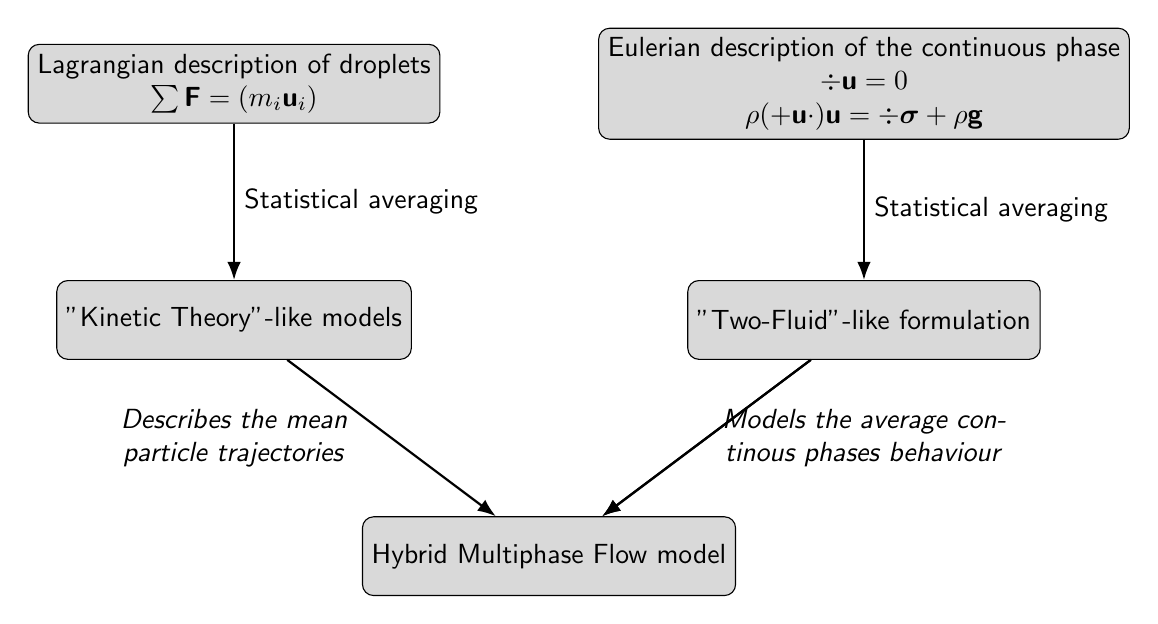
\begin{tikzpicture}
  [
  node distance=3cm and 5cm,
  every node/.style={align=center, font=\sffamily},
  box/.style={draw, rounded corners, minimum width=3.5cm, minimum height=1cm, text centered},
  arrow/.style={-{Latex}, thick},
]

% Nodes
\node[box, fill=gray!30] at (0,3)                                               (lagrangian) {Lagrangian description of droplets \\ $\sum \textbf{F} = \ddt (m_i\textbf{u}_i)$};
\node[box, fill=gray!30] at (8,3)                                               (Eulerian) {Eulerian description of the continuous phase \\ $\div\textbf{u}= 0$\\ $\rho (\pddt + \textbf{u}\cdot\grad)\textbf{u} = \div\bm\sigma + \rho\textbf{g} $};
\node[box, fill=gray!30] at (0,0)                                               (kinetic) {"Kinetic Theory"-like models};
\node[box, fill=gray!30] at (8,0)                             (twofluid) {"Two-Fluid"-like formulation};
\node[box, fill=gray!30] at (4,-3)                           (unify)  {Hybrid Multiphase Flow model};

% Arrows
\draw[arrow] (lagrangian) -- (kinetic) node[midway, right] {Statistical averaging};
\draw[arrow] (Eulerian) -- (twofluid) node[midway, right] {Statistical  averaging};
\draw[arrow] (twofluid) -- (unify);% node[midway, above right] {Mesoscale closures};
\draw[arrow] (kinetic) -- (unify);% node[midway, above left] {Statistical averaging\\(macroscale)};
\draw[arrow] (twofluid) -- (unify);% node[midway, above right] {Mesoscale closures};

% Supporting explanations
\node[below =0.5cm of kinetic, text width=4.5cm] (desc1) {\textit{Describes the mean particle trajectories}};
\node[below =0.5cm of twofluid, text width=4.5cm] (desc2) {\textit{Models the average continous phases behaviour}};

\end{tikzpicture}

\end{frame}

\begin{frame}{Lagrangian's description of fluid particles for kinetic-theory}
  Most of the existing ``hybrid'' model are developed for \textbf{Solid spherical particles' suspension}. 
  \begin{itemize}
    \item What is the difference with classical solid particule models? (R. Jackson 1997, D.Z. Zhang and A. Prosperetti 1997)
    \item How does the surface tension play a role in the conservation equations? 
    \item How to model non-spherical and deforming particules?
  \end{itemize}  
  \pause
  \underline{More importantly :}
  \begin{itemize}
    \item What are the models needed to feed the ``Hybrid-model''  for modeling of emulsions. 
  \end{itemize}
\end{frame}


\begin{frame}
  \frametitle{Mettre main restuls}

  

\end{frame}
\section{Direct Numerical Simulation (DNS) of buoyant emulsions}
\section*{}

\begin{frame}
  \frametitle{Direct Numerical Simulation of buoyant emulsions}
  \begin{columns}
    \column{0.6\textwidth}
  \underline{Simulation set up :} 
  \begin{itemize}
  \item Tri-periodic boundary conditions.
  \item Buoyancy only.
  \item \textbf{Mono-disperse} distribution of droplet size.
  \item We prevent (VOF) coalescence using a special algorithm 
    (\href{http://basilisk.fr/src/no-coalescence.h}{no-coalescence.h})
  \item Free Software: \url{http://basilisk.fr}
  \end{itemize}
  
  \begin{figure}
    \caption{Snapshot of a simulation at $T_g = 300$ for $\phi = 0.01$, $Ga = 75$, $\mu_r = 0.1$ and $N_b = 125$. In white, the interfaces ; the background color map corresponds to the pressure field. The grid represents the different parallel cores.
    }
  \end{figure}
  \column{0.5\textwidth}
  \centering
  \href{file:///work/fintzin/BUBLLES_PROJECT/movies/layers.mp4}{\beamergotobutton{Play}}
  \includegraphics[width =  1.1\textwidth]{image/PHI_01_Ga_75.png}
  \end{columns}
  \end{frame}
  
  \begin{frame}
    \frametitle{Direct Numerical Simulation of buoyant emulsions}
    \begin{columns}
      \column{0.6\textwidth}
    \underline{Dimensionless parameters:} 
    \begin{itemize}
      \item \textit{Galileo} number: $Ga =\frac{\sqrt{\rho_f \Delta\rho_f gD^3}}{\mu} \in [5, 100]$
      \item \textit{Bond} number: $Bo = \frac{\Delta \rho_f g D^2}{\sigma} = 0.2$ 
      \item Volume fraction of dispersed phase: $\phi = [0.01;0.2]$. 
      \item Density and viscosity ratio, $\zeta=\rho_d/\rho_f=0.9$ and $\lambda=\mu_d/\mu_f= 10,1,0.1$. 
    \end{itemize}
    
  \begin{figure}
    \caption{Snapshot of a simulation at $T_g = 300$ for $\phi = 0.01$, $Ga = 75$, $\mu_r = 0.1$ and $N_b = 125$. In white, the interfaces ; the background color map corresponds to the pressure field. The grid represents the different parallel cores.
    }
  \end{figure}
  \column{0.5\textwidth}
  \centering
  \includegraphics[width =  1.1\textwidth]{image/PHI_01_Ga_75.png}
    \end{columns}
\end{frame}
  
  


\section{Characterization of the microstructure}
\section*{}

% \begin{frame}
%   \frametitle{Motivation for studying microstructure}

%   Study of the microstructure  $=$ analysis of the various arrangements and relative motion that droplets can adopt within
%   dispersed buoyant emulsions. 

%   Motivation: 
%   \begin{enumerate}
%     \item Obtain a better physical understanding of what is acctually happening at the local level
%     \item Coalescence Kernels in Population balence equation
%     \item 
%   \end{enumerate}

% \end{frame}

\begin{frame}
  \frametitle{How to describe pair interactions and microstructure?}
  % To better model the film drainage problem we need a clear understanding of How the interactions between droplets works. 
  
  \textbf{Nearest Particule Statistics (Duan Z. Zhang, JFM, 2021): }
  \begin{definition}
    \begin{itemize}
      % \item Let $\mathscr{C} =\left\{\textbf{x}_1, \textbf{r}, \textbf{w},a\right\}$ be the vector containing the position of a particule $\textbf{x}_1$, its nearest neighboring particule relative position $\textbf{r}$, the relative velocity \textbf{w} and the age of the pair time interaction $a$.
      \item Then, $P_{nst}(\textbf{x},\textbf{r},\textbf{w},a) $ is the probability of finding a particule at \textbf{x} with its nearest neighboring particule at \textbf{r} with a relative velocity of \textbf{w} and an age $a$. 
      \item The age $a$ is the time from which a droplet become the nearest neighbor to the current time. 
    \end{itemize}
  \end{definition}

  \begin{align*}
    P_{nst}[\textbf{x},\textbf{r},\textbf{w},a]
    &= \int \Pi[\textbf{x},\textbf{r},\textbf{w},a,\FF] d\FF\\
    (\textbf{f}^\text{nst}P_{nst})[\textbf{x},\textbf{r},\textbf{w},a]
    &= \int (\textbf{f} \Pi)[\textbf{x},\textbf{r},\textbf{w},a,\FF] d\FF
  \end{align*}
  \begin{itemize}
    \item 
    where $\Pi = 1$ if and only if a particule is present at \textbf{x} with its nearest neighbor at \textbf{r} = $\textbf{y}-\textbf{x}$, having an age of $a$ with relative velocity \textbf{w}. 
    \item $\textbf{f}$ can be a Lagrangian property of teh particle or an Eulerian property of the continuous phase. 
  \end{itemize}
\end{frame}

\begin{frame}
  \frametitle{From a 3D distribution to a  2D representation}

  \begin{tikzpicture}
    % \includegraphics{}
    % \node (img2) at (0,0) {\includegraphics[height=0.5\textwidth]{image/pdf_nico.png}};
    \node (img2) at (0,0) {\includegraphics[height=0.5\textwidth]{image/pdf_nico2.png}};
    \node (3D) at (img2.south){3D nearest pair pdf:  $P_\text{nst}(\textbf{r})$};
    \node (img) at (0.5\textwidth,0) {\includegraphics[height=0.3\textwidth]{image/HOMOGENEOUS_NEW/Dist/Pnst_l_1_Ga_100_PHI_0_05.pdf}};
    \draw[red,very thick] (img.south west) rectangle (img.north east);
    \draw[very thick,->] (img2) --(img);
    % \node (2D) at (img.south){$P_\text{nst}(r,\theta)$};
    \node[below= 0.5cm of img] {2D pdf in polar coordinate $P_\text{nst}(r,\theta)$};
  \end{tikzpicture}

\end{frame}
\begin{frame}
  \frametitle{Nearest pair Probability Density Function}

  \begin{columns}
    \column{0.7\textwidth}
    \centering
    \begin{tabular}{cccc}
      &
      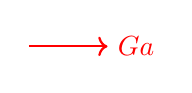
\begin{tikzpicture}[color=red]
        \draw[thick,->] (0,0) -- (1,0)node[right]{$Ga$};
      \end{tikzpicture}& & \\ 
        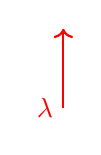
\begin{tikzpicture}[color=red]
          \draw[thick,<-] (0,0) -- (0,-1)node[left]{$\lambda$};
        \end{tikzpicture} 
        &
        \includegraphics[height=0.3\textwidth]{image/HOMOGENEOUS_NEW/Dist/Pnst_l_10_Ga_10_PHI_0_05.pdf}  &
        % \includegraphics[height=0.3\textwidth]{image/HOMOGENEOUS_NEW/Dist/Pnst_l_1_Ga_50_PHI_0_05.pdf} &
        \includegraphics[height=0.3\textwidth]{image/HOMOGENEOUS_NEW/Dist/Pnst_l_10_Ga_100_PHI_0_05.pdf} 
        \\
         &
          \includegraphics[height=0.3\textwidth]{image/HOMOGENEOUS_NEW/Dist/Pnst_l_1_Ga_10_PHI_0_05.pdf} &
        % \includegraphics[height=0.3\textwidth]{image/HOMOGENEOUS_NEW/Dist/Pnst_l_1_Ga_50_PHI_0_05.pdf}&
        \includegraphics[height=0.3\textwidth]{image/HOMOGENEOUS_NEW/Dist/Pnst_l_1_Ga_100_PHI_0_05.pdf}\\
      \end{tabular}

      \column{0.3\textwidth}
      \begin{figure}
        \caption{Plots of $P_{nst} (\textbf{r})$ for different $Ga$ and $\phi$.}
      \end{figure}
    
    \begin{itemize}
      \item Drafting-Kissing-Tumbling mechanism for low $\lambda$ and high $Ga$. 
    \end{itemize}
  \end{columns}
  $\to$ The viscosity ratio $\lambda$ greatly influences the microstructure
\end{frame}

\begin{frame}
  \frametitle{Consequence on the particule arrangements}

  \begin{figure}[h!]
    \centering
    \includegraphics[width=0.45\textwidth]{image/HOMOGENEOUS_NEW/P_PHI_5_l_10_Ga_100.png}
    \includegraphics[width=0.45\textwidth]{image/HOMOGENEOUS_NEW/P_PHI_5_l_1_Ga_100.png}
 %    \includegraphics[width=0.45\textwidth]{image/HOMOGENEOUS_NEW/Ga_100_phi_005_l_10.png}
    \caption{Snapshot of a simulation at $t^* = 150$ for $\phi=0.05$ and $Ga=100$.
      Color map: values of the vertical component of the velocity field on the vertical plane at $z=0$.
      \break
    (left)  $\lambda = 1$.
    (right)  $\lambda = 10$.
    }
    \label{fig:images}
 \end{figure}

\end{frame}


\begin{frame}
  {A concise way to describe the microstructure}
\footnotesize
  We use the second moment of the pair distribution: 
  \begin{align*}
    \textbf{R} = \int \textbf{rr} P_{nst}(\textbf{r}) d\textbf{r}
    &&
    \textbf{A} = 
    \textbf{R} - \frac{1}{3}(\textbf{R}: \bm\delta) \bm\delta
  \end{align*}

%   \begin{figure}
%   \centering
%   \begin{tikzpicture}
    
%   \foreach \i in {1,...,5} {
%   \pgfmathsetmacro{\x}{rnd*0.7}
%   \pgfmathsetmacro{\y}{rnd*0.3}
%   \draw[fill=gray] ($(\x,\y)$) circle (0.1);
%   }
%   \foreach \i in {1,...,5} {
%   \pgfmathsetmacro{\x}{rnd*0.7}
%   \pgfmathsetmacro{\y}{rnd*0.3}
%   \draw[fill=gray] ($(\x+2,\y)$) circle (0.1);
%   }
%   \foreach \i in {1,...,5} {
%   \pgfmathsetmacro{\x}{rnd*0.6}
%   \pgfmathsetmacro{\y}{rnd*0.4}
%   \draw[fill=gray] ($(\x+1,\y-1)$) circle (0.1);
%   }
%   \foreach \i in {1,...,5} {
%   \pgfmathsetmacro{\x}{rnd*0.6}
%   \pgfmathsetmacro{\y}{rnd*0.4}
%   \draw[fill=gray] ($(\x-1,\y-1)$) circle (0.1);
%   }
%   \draw (1,-1)node[below]{$\text tr(\textbf {R}) \ll 1$};

%     \foreach \i in {1,...,20} {
%       \pgfmathsetmacro{\x}{rnd*4}
%       \pgfmathsetmacro{\y}{rnd*2}
%       \draw[fill=gray] ($(\x+5,\y-1)$) circle (0.1);
%       }
%       \draw (6.5,-1)node[below]{$\text tr(\textbf {R})/r_m^2 < 1$};
%     \end{tikzpicture}
%     \hfill
% \end{figure}
\begin{figure}
  \centering
  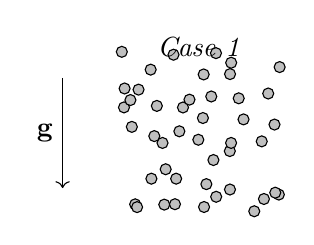
\begin{tikzpicture}[scale=0.7]
  \draw[->] (-1,2.5)--++(0,-2)node[midway, left]{$\textbf{g}$};
  \foreach \i in {1,...,5} {
  \pgfmathsetmacro{\x}{rnd}
  \pgfmathsetmacro{\y}{rnd}
  \draw[fill=gray!50] ($(\x,\y)$) circle (0.1);
  }
  \foreach \i in {1,...,5} {
  \pgfmathsetmacro{\x}{rnd}
  \pgfmathsetmacro{\y}{rnd}
  \draw[fill=gray!50] ($(\x+1,\y)$) circle (0.1);
  }
  \foreach \i in {1,...,5} {
  \pgfmathsetmacro{\x}{rnd}
  \pgfmathsetmacro{\y}{rnd}
  \draw[fill=gray!50] ($(\x+2,\y)$) circle (0.1);
  }
  \foreach \i in {1,...,5} {
      \pgfmathsetmacro{\x}{rnd}
      \pgfmathsetmacro{\y}{rnd}
      \draw[fill=gray!50] ($(\x+1,\y+1)$) circle (0.1);
  }
  \foreach \i in {1,...,5} {
  \pgfmathsetmacro{\x}{rnd}
  \pgfmathsetmacro{\y}{rnd}
  \draw[fill=gray!50] ($(\x+2,\y+1)$) circle (0.1);
  }
  \foreach \i in {1,...,5} {
  \pgfmathsetmacro{\x}{rnd}
  \pgfmathsetmacro{\y}{rnd}
  \draw[fill=gray!50] ($(\x,\y+1)$) circle (0.1);
  }
  \foreach \i in {1,...,5} {
      \pgfmathsetmacro{\x}{rnd}
      \pgfmathsetmacro{\y}{rnd}
      \draw[fill=gray!50] ($(\x+1,\y+2)$) circle (0.1);
  }
  \foreach \i in {1,...,5} {
  \pgfmathsetmacro{\x}{rnd}
  \pgfmathsetmacro{\y}{rnd}
  \draw[fill=gray!50] ($(\x+2,\y+2)$) circle (0.1);
  }
  \foreach \i in {1,...,5} {
  \pgfmathsetmacro{\x}{rnd}
  \pgfmathsetmacro{\y}{rnd}
  \draw[fill=gray!50] ($(\x,\y+2)$) circle (0.1);
  }
  \draw (1.5,3.4)node[below]{\textit{Case 1}};
\end{tikzpicture}
\hfill
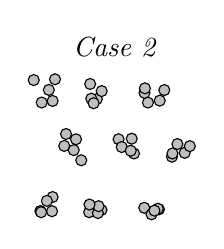
\begin{tikzpicture}[scale=0.7]
  \foreach \i in {1,...,5} {
  \pgfmathsetmacro{\x}{rnd*0.4}
  \pgfmathsetmacro{\y}{rnd*0.4}
  \draw[fill=gray!50] ($(\x,\y)$) circle (0.1);
  }
  \foreach \i in {1,...,5} {
  \pgfmathsetmacro{\x}{rnd*0.3}
  \pgfmathsetmacro{\y}{rnd*0.3}
  \draw[fill=gray!50] ($(\x+1,\y)$) circle (0.1);
  }
  \foreach \i in {1,...,5} {
  \pgfmathsetmacro{\x}{rnd*0.3}
  \pgfmathsetmacro{\y}{rnd*0.3}
  \draw[fill=gray!50] ($(\x+2,\y)$) circle (0.1);
  }
  \foreach \i in {1,...,5} {
      \pgfmathsetmacro{\x}{rnd*0.5}
      \pgfmathsetmacro{\y}{rnd*0.5}
      \draw[fill=gray!50] ($(\x+0.5,\y+1)$) circle (0.1);
  }
  \foreach \i in {1,...,5} {
      \pgfmathsetmacro{\x}{rnd*0.4}
      \pgfmathsetmacro{\y}{rnd*0.4}
      \draw[fill=gray!50] ($(\x+2.5,\y+1)$) circle (0.1);
  }
  \foreach \i in {1,...,5} {
      \pgfmathsetmacro{\x}{rnd*0.4}
      \pgfmathsetmacro{\y}{rnd*0.4}
      \draw[fill=gray!50] ($(\x+1.5,\y+1)$) circle (0.1);
      }
  \foreach \i in {1,...,5} {
      \pgfmathsetmacro{\x}{rnd*0.5}
      \pgfmathsetmacro{\y}{rnd*0.5}
      \draw[fill=gray!50] ($(\x,\y+2)$) circle (0.1);
  }
  \foreach \i in {1,...,5} {
      \pgfmathsetmacro{\x}{rnd*0.4}
      \pgfmathsetmacro{\y}{rnd*0.4}
      \draw[fill=gray!50] ($(\x+2,\y+2)$) circle (0.1);
  }
  \foreach \i in {1,...,5} {
      \pgfmathsetmacro{\x}{rnd*0.4}
      \pgfmathsetmacro{\y}{rnd*0.4}
      \draw[fill=gray!50] ($(\x+1,\y+2)$) circle (0.1);
      }
  \draw (1.5,3.4)node[below]{\textit{Case 2}};
\end{tikzpicture}
\hfill
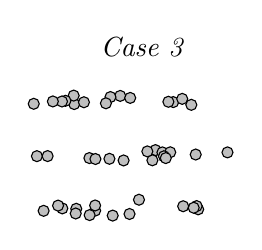
\begin{tikzpicture}[scale=0.7]
  \foreach \i in {1,...,5} {
  \pgfmathsetmacro{\x}{rnd*1.5}
  \pgfmathsetmacro{\y}{rnd*0.2}
  \draw[fill=gray!50] ($(\x,\y)$) circle (0.1);
  }
  \foreach \i in {1,...,5} {
  \pgfmathsetmacro{\x}{rnd*1.5}
  \pgfmathsetmacro{\y}{rnd*0.3}
  \draw[fill=gray!50] ($(\x+1,\y)$) circle (0.1);
  }
  \foreach \i in {1,...,5} {
  \pgfmathsetmacro{\x}{rnd*1.5}
  \pgfmathsetmacro{\y}{rnd*0.3}
  \draw[fill=gray!50] ($(\x+2,\y)$) circle (0.1);
  }
  \foreach \i in {1,...,5} {
      \pgfmathsetmacro{\x}{rnd*1.5}
      \pgfmathsetmacro{\y}{rnd*0.2}
      \draw[fill=gray!50] ($(\x+1+0.5,\y+1)$) circle (0.1);
  }
  \foreach \i in {1,...,5} {
  \pgfmathsetmacro{\x}{rnd*1.5}
  \pgfmathsetmacro{\y}{rnd*0.2}
  \draw[fill=gray!50] ($(\x+2+0.5,\y+1)$) circle (0.1);
  }
  \foreach \i in {1,...,5} {
  \pgfmathsetmacro{\x}{rnd*1.5}
  \pgfmathsetmacro{\y}{rnd*0.1}
  \draw[fill=gray!50] ($(\x+0.5,\y+1)$) circle (0.1);
  }
  \foreach \i in {1,...,5} {
      \pgfmathsetmacro{\x}{rnd*1.5}
      \pgfmathsetmacro{\y}{rnd*0.2}
      \draw[fill=gray!50] ($(\x+1,\y+2)$) circle (0.1);
  }
  \foreach \i in {1,...,5} {
  \pgfmathsetmacro{\x}{rnd*1.5}
  \pgfmathsetmacro{\y}{rnd*0.2}
  \draw[fill=gray!50] ($(\x+2,\y+2)$) circle (0.1);
  }
  \foreach \i in {1,...,5} {
  \pgfmathsetmacro{\x}{rnd*1.5}
  \pgfmathsetmacro{\y}{rnd*0.1}
  \draw[fill=gray!50] ($(\x,\y+2)$) circle (0.1);
  }
  \draw (1.5,3.4)node[below right]{\textit{Case 3}};
\end{tikzpicture}
% \hfill
% \caption{
%   Sketch of the three different particule arrangements identified in this study.
% The gray disks represent droplets in a three-dimensional space.
% Gravity acts in the vertical direction.

% }
% \label{fig:scheme_clusters}
\end{figure}
% \begin{itemize}
%   \item (\textit{Case 1: ``homogeneous''}) A homogeneous arrangement of droplets is called a homogeneous microstructure or just ``homogeneous''.
%   \item (\textit{Case 2: ``clusters''}) Isotropic non-homogeneous microstructure where we observe the presence of ``clusters'' meaning that the particules are close to each other on average.
%   The opposite scenario, where particules are, on average, far from each other, also falls into this category.
%   \item (\textit{Case 3: ``layers''}) The non-isotropic non-homogeneous microstructure where we observe the presence of stratified arrangements.
%   This type of microstructure is referred to as layered microstructure or just ``layers''.
% \end{itemize}
\begin{table}[h!]
  \caption{Microstructure classification}
  \label{tab:microstructure}
  \centering
  \begin{tabular}{|lccccc|} \hline
      Microstructure types & Homogeneous & Isotropic & Figure & $\textbf{R}:\bm\delta/r_m^2$ & $A_{xx}/tr(\textbf{R})$ \\
      Homogeneous & Yes & Yes &(\textit{Case 1}) & $ \approx 1$ & $\approx 0$ \\
      Dispersed &  No & Yes  &(\textit{Case 2}) & $ > 1$ & $\approx 0$ \\
      Clustering &  No & Yes  &(\textit{Case 2}) & $ < 1$ & $\approx 0$ \\
      Layering &    No & No  &(\textit{Case 3}) & $ - $ & $< 1$\\ \hline
  \end{tabular}
\end{table}

\end{frame}


\begin{frame}
  \frametitle{Phase diagram of the microstructure anisotropy}
  \footnotesize
  % \begin{align*}
  %   \textbf{R} = \int \textbf{rr} P_{nst}(\textbf{r}) d\textbf{r}
  %   &&
  %   \textbf{A} = 
  %   \textbf{R} - \frac{1}{3}(\textbf{R}: \bm\delta) \bm\delta
  % \end{align*}
  \begin{figure}[h!]
    \centering
    % \begin{tikzpicture}[scale=0.5]
    %     \node (img) at (0,0) {\includegraphics[height=0.3\textwidth]{image/HOMOGENEOUS_NEW/PA/phase_Rtr_l_1.pdf}};
    %     % \draw[dashed] (10cm,-1.6) ellipse (3 and 2);
    %     \node (txt) at (-2,1) {Clustering};
    %     \node (txt) at (-1,-1.6) {Dispersed};
    %     \draw[dashed] ($(-1,-1.6) + (-10:3 and 2)$(P) arc
    %     (-10:155:3 and 2);
    %     \node (img) at (10.5,0) {\includegraphics[height=0.3\textwidth]{image/HOMOGENEOUS_NEW/PA/phase_Rtr_l_10.pdf}};
    %     % \draw[dashed] (10cm,-1.6) ellipse (3 and 2);
    %     \node (txt) at (8.5,1) {Clustering};
    %     \node (txt) at (10,-1.6) {Dispersed};
    %     \draw[dashed] ($(10,-2) + (-10:3 and 2)$(P) arc
    %     (-10:180:3 and 2);
    % \end{tikzpicture}
    \begin{tikzpicture}[scale=0.5]
        \node (img) at (0,0) {\includegraphics[height=0.3\textwidth]{image/HOMOGENEOUS_NEW/PA/phase_axx_l_1.pdf}};
        \draw[dashed] (1.4,0.3) ellipse (1.5 and 2.5);
        \node (txt) at (1.4,1) {Anisotropic};
        \node (txt) at (-2,1) {Isotropic};

        \node (img) at (10.5,0) {\includegraphics[height=0.3\textwidth]{image/HOMOGENEOUS_NEW/PA/phase_axx_l_10.pdf}};
        % \draw[dashed] (11.7,-0.5) ellipse (0.75 and 1.75);
        % \node (txt) at (11.7,1) {Anisotropic};
        \node (txt) at (8,1) {Isotropic};
    \end{tikzpicture}
    \caption{
        % (top) Phase diagram of the dimensionless mean square distance to the nearest neighbor, $\bm\delta:\textbf{R}/r_m^2$.
         Phase diagram of the dimensionless horizontal components of the anisotropy tensor, $A_{xx}/\text{tr}(\textbf{R})$.  
        (left) Iso-viscosity emulsion $\lambda = 1$.
        (right) Viscous droplets $\lambda = 10$. }
    \label{fig:phase}
\end{figure}

$\to$ Iso-viscosity emulsions exhibit anisotropic clusters at $Ga > 25$ and $\phi \ge 0.05$.  

\end{frame}

\begin{frame}
  {A transport equation to describe the evolution of the microstructure}
  We could show that $\textbf{R}$ obeys the transport equation: 
\begin{equation*}
    \pddt (n_p\textbf{R})
    + \div [
      n_p(\textbf{u}_p\textbf{R}
    + \textbf{R}^\text{Re})]
    = 
    - \frac{n_p\textbf{R}}{a_p}
    +n_p\textbf{B}
    + n_p\textbf{D}
    + n_p\textbf{W}
\end{equation*}
With the ``relative velocity production term''
\begin{align*}
    % n_p \textbf{R}^\text{Re}(\textbf{x},t)
    % =
    % \int_{0}^\infty
    % \int_{\mathbb{R}^3}
    % \textbf{rr}(\textbf{u}^\text{nst}_p - \textbf{u}_p)
    % P(\textbf{x},\textbf{r},t,a)
    % d\textbf{r}da,\\
    % n_p \textbf{B}(\textbf{x},t)
    % =
    % \int_{0}^\infty
    % \int_{\mathbb{R}^3}
    % \textbf{rr}
    % P(\textbf{x},\textbf{r},t,0)\delta(a)
    % d\textbf{r}da, \\
    % n_p\textbf{D}(\textbf{x},t) = 
    % \int_{0}^\infty
    % \int_{\mathbb{R}^3} \textbf{rr}
    % \left[
    %     \frac{1}{a_p(\textbf{x},t)}
    %     - \frac{1}{\tau^\text{nst}(\textbf{x},\textbf{r},t,a)}
    % \right]
    % P_\text{nst}
    % d\textbf{r}
    % da,\\
    n_p \textbf{W}(\textbf{x},t) = 
    \int_{0}^\infty
    \int_{\mathbb{R}^3} \left[
        \textbf{r} \textbf{w}^\text{nst}_p
        + \textbf{w}^\text{nst}_p\textbf{r}
    \right]P_\text{nst}
    d\textbf{r}
    da.
\end{align*} 

\begin{itemize}
  \item  $\textbf{w}^\text{nst}_p(\textbf{x},\textbf{r},t,a)$ is the averaged relative velocity between two nearest neighboring particules, one of which is situated at $\textbf{x}$ and time $t$, with its nearest neighbor at $\textbf{x}+\textbf{r}$ with age $a$. 
  \item \textbf{R} relaxes on a timescale $a_p$ which is related to the particule interaction time.
\end{itemize}

$\to$ The relative approach velocity $\textbf{w}^\text{nst}_p$, and the mean age of interaction $a_p$ seems primordial in the evolution of \textbf{R}. 

\end{frame}


\begin{frame}{Mean time of interaction between droplets}
  \begin{figure}[h!]
    \centering
    \includegraphics[height = 0.3\textwidth]{image/HOMOGENEOUS_NEW/PA/age.pdf}
    % \includegraphics[height = 0.3\textwidth]{image/HOMOGENEOUS_NEW/PA/Corr.pdf}
    % \includegraphics[height = 0.3\textwidth]{image/HOMOGENEOUS_NEW/Dist/Pa_l_1_Ga_10.pdf}
    % \includegraphics[height = 0.3\textwidth]{image/HOMOGENEOUS_NEW/Dist/Pa_l_1_Ga_100.pdf}
    \caption{
    (left) Mean dimensionless age $a_p =  \int_0^\infty aP_a(\textbf{x},t,a)da$ in terms of the \textit{Galileo} number for different volume fraction :   
    ($\pmb\bigcirc$) $\phi = 0.01$; ($\pmb\triangle$) $ \phi = 0.05$; ($\pmb\square$) $\phi = 0.1$ ($\pmb\lozenge$) $\phi = 0.2$.
    The hollow symbols correspond to $\lambda = 1$, the filled symbols to $\lambda = 10$.
    Black symbols represent the DNS results of (Zhang et al. (2023)) for hard sphere suspension with $\phi = 0.0168,0.0565,0.1341,0.2622$, corresponding to the symbols : $\pmb\times, \pmb +, \pmb\star , \pmb\triangledown$, respectively.
    }
    \label{fig:tau_p}
\end{figure}
\end{frame}

\begin{frame}{Relative normal approach velocity}
  \begin{figure}[h!]
    \centering
    % \includegraphics[height = 0.4\textwidth]{image/HOMOGENEOUS_NEW/Age_cond/uR_rel.pdf}
    % \includegraphics[height = 0.3\textwidth]{image/HOMOGENEOUS_NEW/Age_cond/r_l_10_PHI_10.pdf}
    \begin{tikzpicture}[ scale = 0.6]
        \node (img) at (-0.7\textwidth,0){\includegraphics[height = 0.4\textwidth]{image/HOMOGENEOUS_NEW/Age_cond/uR_rel2.pdf}};
        \filldraw[ gray!50!white](0,0) circle (0.5);
        \filldraw[ gray!50!white](1,3)circle (0.5);
        % \draw[fill=gray,opacity=0.2](5,-0.2)circle (0.5);
        % \draw[fill=gray,opacity=0.2](-3,2)circle (0.5);
        % \draw[fill=gray,opacity=0.2](-5,0.2)circle (0.5);
        \draw(0,0)node[right]{$\textbf{x}_i$};
        \draw[dashed](0,0)--(1,3)node[right]{$\textbf{x}_j$};
        % \draw[very thick,<-,blue](-1,0)--++(0,1)node[right]{$\bm{b}$};
        \draw[very thick,->](1,3)--++(0.9,-1.8)node[above right]{$\textbf{w}^\text{nst}(a)$};
        \draw[very thick,->,red](1,3)--++(-0.5,-1.5)node[left]{$w_{ij,n}(a)$};
        \draw[dashed](1,3)++(0.9,-1.8) -- (1,3)++(-0.5,-1.5);
        \node (ii) at (1,-1){$\textbf{w}_{ij} = \textbf{u}_j - \textbf{u}_i$};
        \node (ii) at (1,-1.6){$w_{ij,n} = \textbf{w}_{ij}\cdot \textbf{r}/|\textbf{r}|$};
        % \draw[very thick,->](0,0)--++(1,0)node[below right]{$\bm{e_x}$};
        % \draw[very thick,->](0,0)--++(0,1)node[left]{$\bm{e_y}$};
        % \draw(3,1)++(199:1)node[above left]{$\beta$} arc(199:159:1);
        % \draw(0,0)++(0:1)node[above right]{$\theta$} arc(0:20:1);
    \end{tikzpicture} 
    % \caption{(left) \textbf{Relative normal approach velocity} between two nearest neighbors, averaged conditionally on the age of interaction.  
    % The age $a$, as well as the velocity are made dimensionless  with the mean age $\tau_a$ and the length scale $d_p = n_p^{-1/3}$. 
    % The symbols represent the different \textit{Galileo} numbers, the colors the different 
    % ($\pmb\bigcirc$) $Ga=10$; ($\pmb\triangle$) $ Ga = 25$; ($\pmb\square$) $Ga = 50$ ($\pmb\lozenge$) $Ga =100$.
    % The colors represent the different volume fractions, (blue) $\phi =0.01$, (green) $\phi = 0.05$ (organ) $\phi=0.1$ (red) $\phi = 0.2$. 
    % The white symbols correspond to $\lambda = 1$, and black symbols to $\lambda = 10$. 
    % (right)
    % Scheme of two nearest neighbors with their position $\textbf{x}_i$ and $\textbf{x}_j$, velocities $\textbf{u}_{i}$ and $\textbf{u}_j$, relative velocity $\textbf{w}_{ij}$ and normal relative velocity $w^{ij,n}$. 
    % (black lines) Semi-empirical formulation .
    % }
    % \label{fig:normal_vel_picture}
\end{figure}
The theoretical observations suggest that in a statistically steady-state regime :
\begin{equation}
\int_\mathbb{R} w_{pn}^aP_a(\textbf{x},t,a) da = 0 
\end{equation}

\end{frame}
\begin{frame}{Relative normal approach velocity}
  \begin{figure}[h!]
    \centering
    % \includegraphics[height = 0.4\textwidth]{image/HOMOGENEOUS_NEW/Age_cond/uR_rel.pdf}
    % \includegraphics[height = 0.3\textwidth]{image/HOMOGENEOUS_NEW/Age_cond/r_l_10_PHI_10.pdf}
    \begin{tikzpicture}[ scale = 0.6]
        \node (img) at (-0.7\textwidth,0){\includegraphics[height = 0.4\textwidth]{image/HOMOGENEOUS_NEW/Age_cond/uR_rel.pdf}};
        \filldraw[ gray!50!white](0,0) circle (0.5);
        \filldraw[ gray!50!white](1,3)circle (0.5);
        % \draw[fill=gray,opacity=0.2](5,-0.2)circle (0.5);
        % \draw[fill=gray,opacity=0.2](-3,2)circle (0.5);
        % \draw[fill=gray,opacity=0.2](-5,0.2)circle (0.5);
        \draw(0,0)node[right]{$\textbf{x}_i$};
        \draw[dashed](0,0)--(1,3)node[right]{$\textbf{x}_j$};
        % \draw[very thick,<-,blue](-1,0)--++(0,1)node[right]{$\bm{b}$};
        \draw[very thick,->](1,3)--++(0.9,-1.8)node[above right]{$\textbf{w}^\text{nst}(a)$};
        \draw[very thick,->,red](1,3)--++(-0.5,-1.5)node[left]{$w_{ij,n}(a)$};
        \draw[dashed](1,3)++(0.9,-1.8) -- (1,3)++(-0.5,-1.5);
        \node (ii) at (1,-1){$\textbf{w}_{ij} = \textbf{u}_j - \textbf{u}_i$};
        \node (ii) at (1,-1.6){$w_{ij,n} = \textbf{w}_{ij}\cdot \textbf{r}/|\textbf{r}|$};
        % \draw[very thick,->](0,0)--++(1,0)node[below right]{$\bm{e_x}$};
        % \draw[very thick,->](0,0)--++(0,1)node[left]{$\bm{e_y}$};
        % \draw(3,1)++(199:1)node[above left]{$\beta$} arc(199:159:1);
        % \draw(0,0)++(0:1)node[above right]{$\theta$} arc(0:20:1);
    \end{tikzpicture} 
    % \caption{(left) \textbf{Relative normal approach velocity} between two nearest neighbors, averaged conditionally on the age of interaction.  
    % The age $a$, as well as the velocity are made dimensionless  with the mean age $\tau_a$ and the length scale $d_p = n_p^{-1/3}$. 
    % The symbols represent the different \textit{Galileo} numbers, the colors the different 
    % ($\pmb\bigcirc$) $Ga=10$; ($\pmb\triangle$) $ Ga = 25$; ($\pmb\square$) $Ga = 50$ ($\pmb\lozenge$) $Ga =100$.
    % The colors represent the different volume fractions, (blue) $\phi =0.01$, (green) $\phi = 0.05$ (organ) $\phi=0.1$ (red) $\phi = 0.2$. 
    % The white symbols correspond to $\lambda = 1$, and black symbols to $\lambda = 10$. 
    % (right)
    % Scheme of two nearest neighbors with their position $\textbf{x}_i$ and $\textbf{x}_j$, velocities $\textbf{u}_{i}$ and $\textbf{u}_j$, relative velocity $\textbf{w}_{ij}$ and normal relative velocity $w^{ij,n}$. 
    % (black lines) Semi-empirical formulation .
    % }
    % \label{fig:normal_vel_picture}
\end{figure}
The theoretical observations suggest that in a statistically steady-state regime :
\begin{equation}
  w_{pn}^a(\textbf{x},t,a) = \frac{d_p}{\tau_p} 
  \left(
      0.15
      -\frac{\phi}{2}
  \right)\left(
      1 - 3e^{-2a/\tau_p}
  \right).
\end{equation}
\end{frame}

\section{Development of closure laws}
\section*{}

\begin{frame}{Closure terms for the momentum averaged equations }
  Averaged \textbf{mass} and \textbf{momentum} equations for the continuous phase :
\begin{align*}
  % \phi_d + \phi_f &= 1\\
  \pddt \phi_f   
  + \div (\phi_f \textbf{u}_f)
  &= 
  0\\
  \rho_f (\pddt + \textbf{u}_f \cdot\grad)\textbf{u}_f
  &= 
  \div\bm\sigma_f^\text{eff}
  + \phi_f  \rho_f \textbf{g}
  + 
  \underbrace{
    n_p \textbf{f}_p
    % \avg{\delta_I \bm{\sigma}_f^0 \cdot \textbf{n}_f}
  }_\text{Interphase drag force}
\end{align*}
With the effective stress : 
\begin{align*}
  &\bm{\sigma}_f^\text{eff}
  = 
   \underbrace{\rho_f\avg{\chi_f \textbf{u}_f'\textbf{u}_f'}}_\text{Reynolds stress}
    - \underbrace{\phi_f \bm{\sigma}_f}_\text{Mean Newtonian stress}
\end{align*}
\begin{itemize}
  \item $\textbf{u}_f$ mean velocity of the continuous phase.  
  \item $\rho_f$ : density of the continuous phase. 
  \item $\phi_f$ : volume fraction of the continuous phase. 
  \item $n_p$ number of particle per unit of volume. 
  \item $\avg{\ldots}$ : the ensemble average operator. 
  \item $\textbf{u}_f' = \textbf{u}^0_f - \textbf{u}_f$ where $\textbf{u}_f^0$ is the local (non-averaged) fluid velocity. 
\end{itemize}
\end{frame}


\begin{frame}
  \frametitle{Drag coefficient model for viscous droplets emulsions}
  % \begin{figure}[h!]
    \centering    
    \includegraphics[height = 0.23\textwidth]{image/HOMOGENEOUS_final/CA/Cp_l_0.pdf}
    \includegraphics[height = 0.23\textwidth]{image/HOMOGENEOUS_final/CA/Cp_l_1.pdf}
    \includegraphics[height = 0.23\textwidth]{image/HOMOGENEOUS_final/CA/Cp_l_10.pdf}
%     \caption{
%         Drag coefficient $C_p$ in term of the Reynolds number $Re$.  
%         The symbols correspond to different volume fraction. 
%     }
%     \label{fig:Cp}
% \end{figure}
% \footnotesize
\begin{equation*}
  \frac{\textbf{f}_p}{\frac{1}{8}\rho_f \pi d^2 U^2}
  = 
  \underbrace{
    \frac{  \textcolor{red}{\lambda}   C_D^\text{Sol}(Re)+ C_D^\text{Bub}(Re)}
    {1+\textcolor{red}{\lambda}} 
    }_\text{Isolated drag force correlation}
    \times
  \underbrace{f_\phi(\phi, Re,\textcolor{red}{\lambda})}_\text{Swarm coefficient}
\end{equation*}
\begin{itemize}
  % \item Creation of a new model which takes in account the viscosity ratio : \textcolor{red}{$\lambda$}. 
  \item $U$, $d$ Mean relative velocity and drop diameter. 
  \item $C_D^\text{Sol}$ is the drag force coefficient on an isolated solid sphere and $C_D^\text{Bub}$ the drag force coefficient on a shear-free bubble
  \item $f_\phi$ Richardson and Zaki law, with an exponant function of $Re$ and $\lambda$. 
  % \item $f_\phi$ Richardson and Zaki law, with an exponant function of $Re$ and $\lambda$. 
\end{itemize}

\end{frame}

\begin{frame}
    {
    Drops induced pseudo turbulence model : 
    }
    \small
    \begin{equation*}
      \avg{\chi_f  \textbf{u}_f' \textbf{u}_f'}
      =
      \underbrace{
        C_1(\phi)\textbf{UU}
      + C_2(\phi)U^2 \bm\delta
      + \overbrace{C_1(\phi)\avg{\textbf{u}_p'\textbf{u}_p'}
      + C_2(\phi)\avg{\textbf{u}_{p}'\cdot \textbf{u}_{p}'}\bm\delta
      }^{\text{Particle center of mass velocity fluctuations}}
      }_\text{Particle Induced Turbulence (PIT)}
      % }_\text{Bubble induced turbulence in a uniform flow}
      % \\
    \end{equation*}
    % \pause
    \begin{equation*}
      + \underbrace{\frac{\phi_d a^2 }{105 (\lambda +1)^2 }\left[
          (129\lambda^2+108\lambda+24)\textbf{E}\cdot \textbf{E}
          + (20\lambda^2 +20\lambda + 6)
          (\textbf{E} : \textbf{E})\bm\delta
      \right]}_\text{Shear Particle Induced Turbulence (S-PIT)}
  \end{equation*}
  % \begin{columns}
    % \column{0.5\textwidth}
    \begin{align*}
      C_{1} = \frac{9(2+3\lambda)^2 \Gamma(1/3)}{80 (\lambda +1)^2}\phi^{2/3} 
      &&
      C_2 = \frac{9(2+3\lambda)^2 \Gamma(1/3)}{80 (\lambda +1)^2}\phi^{2/3} 
      % - \frac{27+82\lambda + 62\lambda^2}{20(\lambda + 1)^2}\phi \right)
    \end{align*}
    \begin{itemize}
      \item $\avg{\textbf{u}_p'\textbf{u}_p'}$ Particles center of mass velocity fluctuation.  
      \item $\textbf{U}$ Mean relative velocity. 
      \item $\textbf{E}$ Mean fluid phase shear rate. 
    \end{itemize}
    % \column{0.2\textwidth}
    % \begin{figure}
    %   \caption{Disturbance velocity field of a droplet immersed in a pure linear flow}
  %   \end{figure}
  %   \column{0.4\textwidth}
  %   \includegraphics[width=0.6\textwidth]{image/Shear_Stokes.png}
  % \end{columns}
\end{frame}

\section{Conclusion and perspectives}
\section*{}

\begin{frame}
  \frametitle{Mettre perspective des procede}

  

\end{frame}

\begin{frame}
  \frametitle{Conclusion and perspectives}

  % \begin{itemize}
  %   \item We used the Nearest Particule Statistics framework to describe the microstructure of dispersed two-phase flow. 
  %   \item We could show that the microstructure can be described qualitatively and quantitatively using the second-order tensor \textbf{R}.
  %   \item An averaged evolution equation for this tensor was derived.
  %   \item The viscosity ratio $\lambda$ has a strong impact on the microstructure. 
  %   % \item We used the nearest particule statistics to derive relative pair interactions equations. 
  %   % \item We found out that relative positions and velocity were directly correlated to the relative position \textbf{r} and age of the interaction $a$, with $Ga$ and $\phi$. and $\lambda$ 
  %     % \item The interaction relaxation time corresponds approximately to the mean age of interaction $\tau =\avg{a}$.
  %   % \item Paper to appear in a special issue of Acta Mechanica.
  % \end{itemize}
  \begin{enumerate}
    \item We derived an ``hybrid'' formulation for the  modeling of dispersed two-phase flow made of arbitrary shaped fluid drops with surface properties. 
    \item We provided a general method to describe the  geometry and kinematics   properties of the microstructure of buoyant rising emulsions using Nearest-Particle-Statistics
    \item We provided semi-empirical closure laws to feed the ``hybrid model'',  including the drag force and Reynolds stress. 
  \end{enumerate}
\vfill    
% \vspace{1cm}
See my work here: \url{http://basilisk.fr/sandbox/fintzin/Rising-suspension/RS.c}

\end{frame}


 \end{document}
